\documentclass{article}

% if you need to pass options to natbib, use, e.g.:
% \PassOptionsToPackage{numbers, compress}{natbib}
% before loading nips_2017
%
% to avoid loading the natbib package, add option nonatbib:
% \usepackage[nonatbib]{nips_2017}

%\usepackage{nips_2017}
\usepackage[final, nonatbib]{nips_2017}

\usepackage[utf8]{inputenc} % allow utf-8 input
\usepackage[T1]{fontenc}    % use 8-bit T1 fonts
\usepackage{hyperref}       % hyperlinks
\usepackage{url}            % simple URL typesetting
\usepackage{booktabs}       % professional-quality tables
\usepackage{amsfonts}       % blackboard math symbols
\usepackage{nicefrac}       % compact symbols for 1/2, etc.
\usepackage{microtype}      % microtypography
% my packages
\usepackage{graphicx}
\usepackage{placeins}
\usepackage{amsmath}
\usepackage{subcaption}

\title{Playing Blackjack with Deep Q-Learning}

\author{
  Allen Wu\\
  Management Science \& Engineering\\
  Stanford University\\
  Stanford, CA 94305 \\
  \texttt{nalkpas@stanford.edu} \\
}

\begin{document}

\maketitle

\begin{abstract}
  Traditional $Q$-learning is a powerful reinforcement learning algorithm for small state-action spaces, but performs poorly on more involved systems. Deep $Q$-learning extends traditional $Q$-learning using a neural network and experience replay buffer and has been proven effective for learning environments as complex as chess [1], go [2], and Atari video games [3]. In this paper, we apply deep $Q$-learning with annealing $\epsilon$-greedy exploration to blackjack, a popular casino game, to test how well the algorithm can learn a probabilistic environment. We find that although deep $Q$-learning dramatically outperforms traditional $Q$-learning and learns an effective policy, it's ultimately unable to find the exact optimal policy. 
\end{abstract}

\section{Introduction}

\subsection{Blackjack}

Blackjack is one of the oldest casino games and remains popular today, though its status has declined as the mathematics of the game have become more widely known. The first record of blackjack is Miguel de Cervantes's 16\textsuperscript{th} century novella \textit{Rinconete y Cortadillo}, whose protagonists cheat at blackjack [4]. The player's goal in blackjack is to acquire a hand whose sum is greater than the sum of the dealer's hand, which is partially hidden, without that sum exceeding 21. The mathematics of blackjack were first studied in the 1950s, when Baldwin et al. published a paper providing a probabilistic solution to the game under some simplifying assumptions [5]. 

Because blackjack is sufficiently complicated that the optimal strategy isn't obvious, it represents an almost purely Markov decision process, and it has a natural reward scheme with a closed-form solution, it's a promising environment for testing the efficacy of reinforcement learning methods.

\subsection{Deep $Q$-Networks} 

Deep $Q$-networks were first introduced in Mnih et al.'s paper \textit{Playing Atari with Deep Reinforcement Learning} [3]. Mnih et al. generalized $Q$-learning to larger state and action spaces by using a neural network to learn the $Q$-matrix rather than storing the $Q$-matrix directly in memory. In addition, they introduced the concept of the experience replay buffer, which stores and samples from the agent's experiences. These two improvements allowed $Q$-learning to learn large state spaces and sparse reward structures much better, reducing the two primary weaknesses of the algorithm. 

Since Mnih et al. first introduced the idea of deep $Q$-networks in 2013, further research has led to breakthroughs such as AlphaGo, the first computer go player capable of competing with top human players [2]. Deep $Q$-networks remain at the forefront of reinforcement learning research to this day. 

\subsection{Deep $Q$-Learning of Blackjack}

In this paper, we apply Mnih et al.'s original deep $Q$-network to blackjack in order to test, explore, and better understand their methods. We implement a state-machine for playing blackjack and train a deep $Q$-network on that state-machine using a variety of different network settings. Our network accepts a blackjack hand as input and outputs a score for each of the five legal actions that approximates the expected reward of taking each. After locally optimizing our hyperparameters, we evaluate our network's final policy by simulating its expected return and finding its similarity to the closed-form optimal policy. We also implement a traditional $Q$-network and train it for 50 million episodes using similar parameters to the deep $Q$-network for comparison.  

\subsection{Related Work}

In addition to Mnih et al.'s seminal \textit{Playing Atari with Deep Reinforcement Learning} [3], we took inspiration from DeepMind's later papers \textit{Mastering the Game of Go with Deep Neural Networks and Tree Search} by Silver and Huang [2] and \textit{Mastering Chess and Shogi by Self-Play with a General Reinforcement Learning Algorithm} by Silver, Hubert, and Schrittweiser [3]. However, these papers primarily addressed multi-player rather than single-player games and the techniques they describe don't fully generalize. 

For implementation, we referred to \textit{Implementing the Deep Q-Network} by Roderick, MacGlashan, and Tellex [6], a survey paper that reviewed a number of implementation details in Mnih et al.'s original deep $Q$-network that the Atari paper glossed over. In addition, we started out following the PyTorch deep reinforcement learning tutorial by Adam Paszke. [7]  

\section{The Blackjack Model}

\subsection{Rules of Blackjack} The dealer begins a hand of blackjack by dealing two cards to the player and two cards to himself. The player can only see one of the dealer's cards. Rules vary from casino to casino, but in the maximal game the player can take five actions: 

\begin{itemize}
	\item \textit{\textbf{Hit}}, to receive another card from the dealer. 
	\item \textit{\textbf{Stand}}, to end the hand. 
	\item \textit{\textbf{Surrender}}, to forfeit the hand and save half of her bet. 
	\item \textit{\textbf{Double}}, where the player doubles her bet, hits, and then stands. 
	\item \textit{\textbf{Split}}, where the player starts two new hands using one of each of her original cards, staking her original bet in each.  
\end{itemize} 

Surrendering and doubling may only be taken as the first action in a hand. Splitting may only be taken when the player has a pair.

The player's hand has value equal to the sum of its cards. All face cards are worth 10 and aces may be counted as either 1 or 11. If a player's hand exceeds 21, she \textbf{breaks}, losing the hand automatically. Hands featuring aces are called \textbf{soft}, because they cannot break while the ace counts for 11. 

After the player stands, the dealer then completes his hand according to the casino \textbf{rule}. In most casinos, the dealer must continue to take cards until his hand is hard 17, soft 18, or greater. If the dealer breaks, the player wins. Otherwise, the player wins if her hand is worth more than the dealer's. The player receives her bet back in case of ties, except when the dealer has \textbf{blackjack}, or when his starting cards sum to 21. In that case, the player loses no matter what her hand is. However, when the dealer has blackjack, the player only loses her original bet no matter what prior actions she took. 

When the player has blackjack herself, she always wins and receives an additional half bet. 

\subsection{State-Action Space}

We aimed to model blackjack as completely as possible, in order to pose the most difficult question we could. We model a hand as a tuple of five characteristics: the player's hand,  the dealer's hand, whether the hand is soft, whether it's the first action in a hand, whether the player's hand is a pair. It's important to track whether a hand has just started both so the state-machine can correctly return the list of legal actions, but also so that the $Q$-network doesn't overvalue hitting to states where doubling is particularly valuable, or underestimate the impact of hitting to states where it would surrender. Tracking whether the hand is paired is valuable for the same reasons: a 12 consisting of two aces that can be split is much more valuable than a 5 and a 7. 

We allow the player all five legal actions. Rather than expanding the state space to accommodate splitting, we model splitting as the player doubling her bet, keeping one of her cards, and starting a new hand. Our split has higher variance than splitting in practice, since we directly correlate the stochasticity in the two hands, but it has the same expectation. The decision to split depends only on the true expectation, which the agent should learn over time. 

\subsection{Rules}

We follow the typical rules of casino blackjack exactly, except we assume an infinite deck and don't account for player blackjack. An infinite deck approximates practice, as most modern casinos use multiple decks that are regularly reshuffled, but most importantly makes simulation simpler and faster. Player blackjack is irrelevant for our purposes because it doesn't require any decisions. 

\section{Methods}

\subsection{Exploration}

We used $\epsilon$-greedy exploration with an annealing $\epsilon$. This facilitates greater exploration at the start of training and greater exploitation towards the end, approximating the effect of more involved exploration algorithms without the additional complexity. This method typically involves scaling $\epsilon$ by a factor of $e^{-t}$ so that $\epsilon$ tends toward $0$ over time, but this causes $\epsilon$ to decrease at an increasing rate. We experimented with a concave $\epsilon$ function so our agent would explore splitting, doubling, and surrendering more aggressively, preventing overfitting. We set $\epsilon = \epsilon_s + (\epsilon_f - \epsilon_s)e^{\frac{t - f}{k}}$, where $\epsilon_s$ and $\epsilon_f$ are starting and ending values of $\epsilon$, $k$ is a scaling factor, and $f$ is the length of the period at the end where we want to maximally exploit. 

To further reduce overfitting, we also use a burn-in period of 50,000 episodes where the agent takes random actions. This follows the Atari model, as noted in Melrose et al. [6] In addition, we restrict the agent from selecting the most promising action when it acts randomly. 

\subsection{Experience Replay}

Some of the major problems of traditional $Q$-learning are that the agent doesn't learn sparse reward schemes very well, can underestimate the value of uncommon actions, and overfits to recent experiences. One of the major innovations in Mnih. et al's original deep $Q$-network was to instead use a experience replay buffer. At fixed time steps, the agent samples a batch of experiences from the buffer and updates from that sample. Old experiences are forgotten when new experiences overflow the buffer. The experience replay buffer both diminishes the impact of new experiences and propagates rare events and rewards more completely through the network. 

We use a buffer length of 20000 experiences and a batch size of 256. Using buffer and batch sizes that are too big can cause the agent to overfit to early experiences. We settled on these numbers after experimenting with various sizes relative to the length of our training. 

\subsection{The Deep $Q$-Network}

Because our state-space consists of sequences of floats and encapsulates all meaningful time-dependencies, it made sense to use a simple fully connected linear network rather than the convolutional models used for image-based games. Following convention, we use batch normalization and ReLU activations in every layer except the last, which is fully linear. We use a small weight decay of $0.0001$ to make sure our parameters don't explode. 

To update our network, we sample a batch of $(s, a, s', r)$ experiences from the memory buffer, calculate $V_{s'} = r + \gamma \max_{a} Q(s', a)$ for each experience in our sample, then update $Q(s)$ using Huber loss with respect to $V_{s'}$. Huber loss, or smooth $L_1$ loss, behaves like $L_2$ loss for $x \in [-1,1]$ and $L_1$ loss elsewhere. It offers greater fidelity for critical values of $x$ but is more resistant to outliers than regular $L_2$ loss. Given we expect most actions to have expected outcomes near $0$ but some extremes, Huber loss is a perfect fit. Again following the implementation in Melrose et al. [6], we take a gradient descent step after every 4 experiences so that we don't update excessively. To update our network, we use stochastic gradient descent with $\beta = 0.9$. 

When calculating $\max_{a} Q(s', a)$, we mask the scores of illegal actions with arbitrarily negative values. This prevents our agent from valuing illegal actions, the scores for which are essentially just noise. We considered severely penalizing our agent for taking illegal actions so that it learns which actions are legal, but ultimately determined that this was functionally equivalent to masking and would make learning unnecessarily more difficult. 

\subsection{Hyperparameters}

For $Q$-learning updates, we use a discount rate of $\gamma = 0.999$ so future rewards are almost equivalent to present rewards. Episodes terminate after relatively few actions anyway and philosophically, the value of money doesn't change in a couple of minutes. After trying learning rates of $0.0001, 0.00001,$ and $0.000001$, we settled on $0.0001$ as even small networks were learning too slowly with the smaller rates. We trained our test networks for 500,000 episodes and our final network for 1,500,000 episodes. 

The two main hyperparameters we tuned were the depth and size of the network, since they seemed like the most important. We parameterized our network using the depth $n$ and a scaling factor $k$, such that the first hidden layer has $kn_{\text{in}}$ nodes and subsequent layers $i$ have $\lceil (\nicefrac{n_{\text{out}}}{kn_{\text{in}}})^{\frac{i - 1}{n - 1}} \rceil$ nodes. This scaling method lets us control the size of our network with a single parameter and ensures that our network has a classical funnel shape, outputting progressively fewer activations. 

We get the following graphs by holding one parameter constant and varying the other: 

\FloatBarrier
\begin{figure}[h]
	\centering
	\begin{subfigure}{0.4\textwidth}
		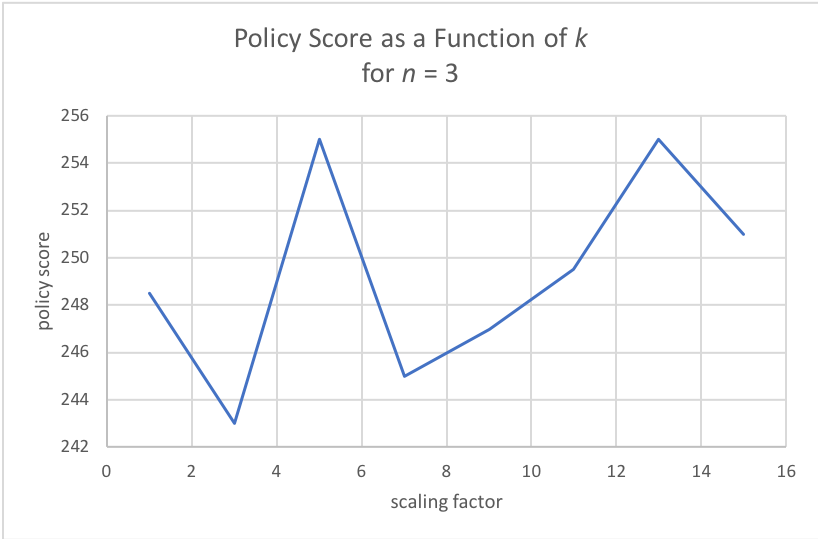
\includegraphics[width=\textwidth]{k_graph}
		\caption{Score as a function of $k$ for $n = 3$}
	\end{subfigure}
	~
	\begin{subfigure}{0.4\textwidth}
		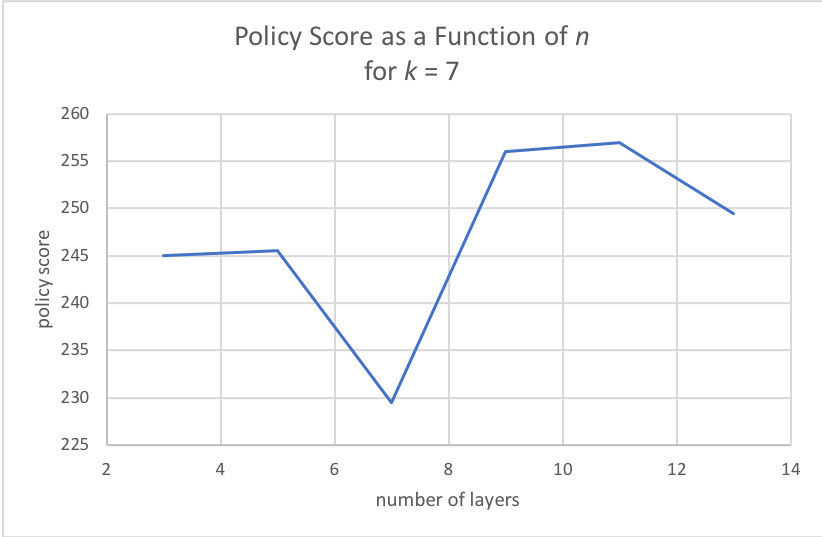
\includegraphics[width=\textwidth]{n_graph}
		\caption{Score as a function of $n$ for $k = 7$}
	\end{subfigure}
\end{figure}
\FloatBarrier

We'll explain our "policy score" metric in more detail in the next section, but it approximates the quality of the final policy. A high policy score is good. We couldn't find a clear relationship between the size of the network and the quality of its predictions, but bigger networks generally performed better. We picked the best performing $k = 13$ and $n = 11$ for our final network.  

\subsection{Evaluation}

We evaluated policies based on two criteria: policy score and expected return.

Policy score is analogous to the similarity between the optimal policy and the network's policy. However, there are gray areas in the blackjack optimal policy where the correct action depends on the casino's exact rules and the number of decks the casino uses. In these gray areas, we award a policy a full point if it dictates the most commonly correct action and a half point if it dictates the second-best action. Policy score is out of 340 points, suggesting a coupled similarity metric. 

Expected return is the mean outcome of the policy. We find this by simulating 5 million hands.  

\section{Results}

We ultimately get the following results, using the notation DQN($n$, $k$) and including some smaller networks as additional baselines: 

\FloatBarrier
\begin{center}
	\begin{tabular}{ c|c|c|c } 
		
		Network & Policy Score & Similarity & Expected Return \\ 
		\hline
		QN & 228.5 & 0.672058824 & -0.26189 \\ 
		DQN(3,1) & 248.5 & 0.730882353 & -0.1140973 \\ 
		DQN(13,7) & 249.5 & 0.733823529 & -0.1218813 \\ 
		DQN(11, 13) & 259.5 & 0.763235294 & -0.107426 \\ 
		optimal policy & 340 & 1 & -0.095752 \\ 
	\end{tabular}
\end{center}
\FloatBarrier

Even though our policy is somewhat dissimilar to the optimal policy, it only loses an additional $0.01167$ bets per hand than the best policy\footnote{A loss of 0.09575 bets per hand is a lot more than the well-cited 1-2\% house edge, but this is because we greatly reduces our player's equity in our model by not factoring in player blackjack and its additional payout.}. This means that even though we often don't learn the best action, we at least learn a good action. Further, we massively outperform a traditional $Q$-network, which is unable to adjust to the expanded state space. Nonetheless, despite all this, our best policy doesn't improve much over our simpler networks and doesn't match the optimal policy well.

We can also analytically compare our derived policy to the optimal policy: 

\FloatBarrier
\begin{figure}[h]
	\centering
	\begin{subfigure}{0.45\textwidth}
		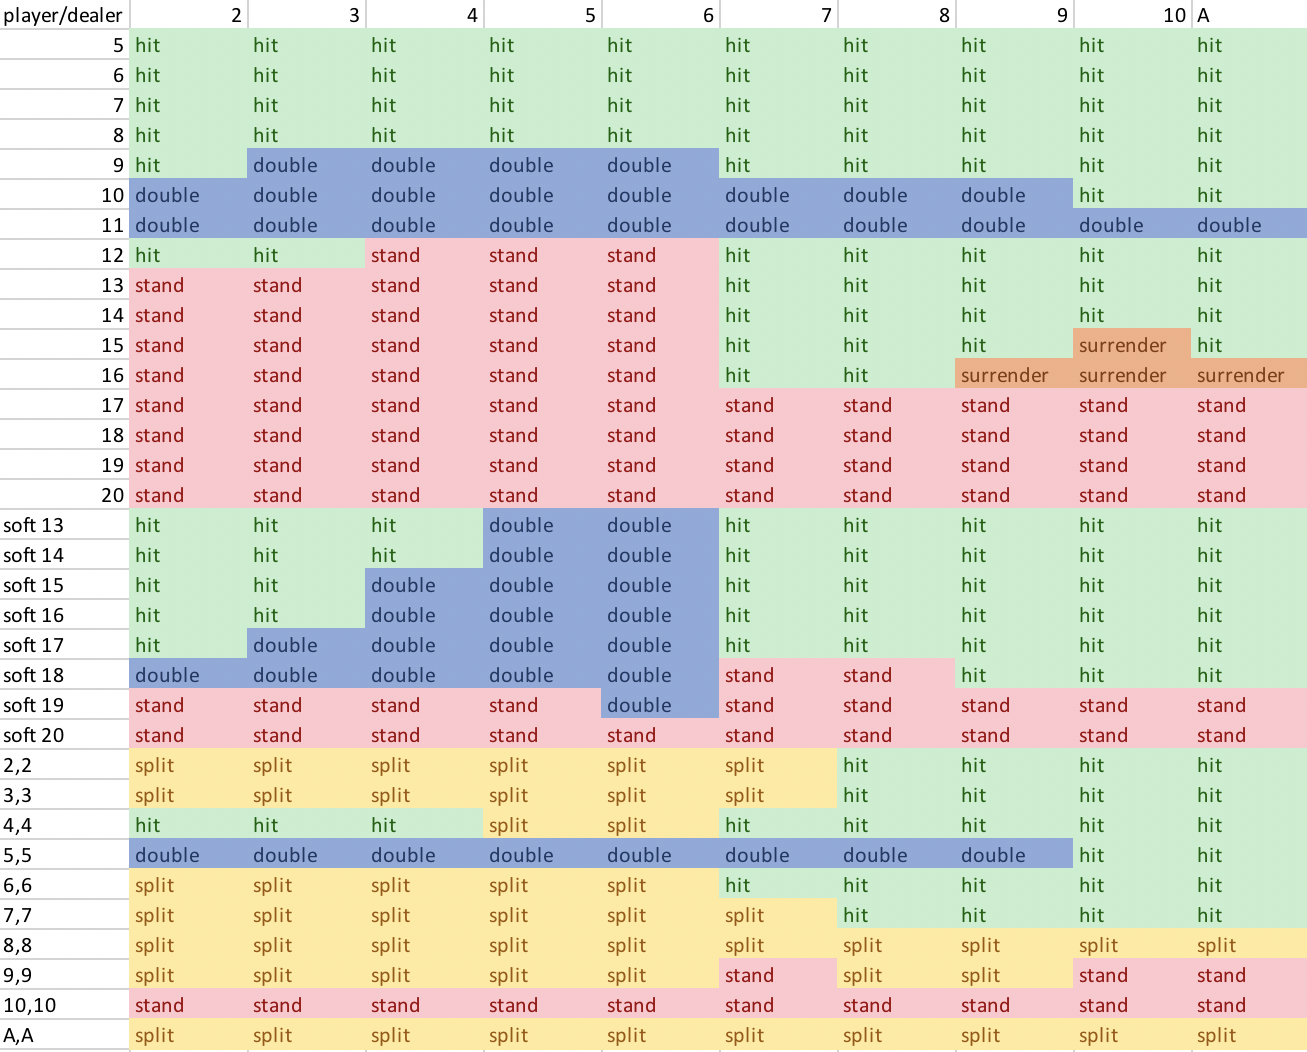
\includegraphics[width=\textwidth]{opt_chart}
		\caption{Optimal policy [4]}
	\end{subfigure}
	~
	\begin{subfigure}{0.45\textwidth}
		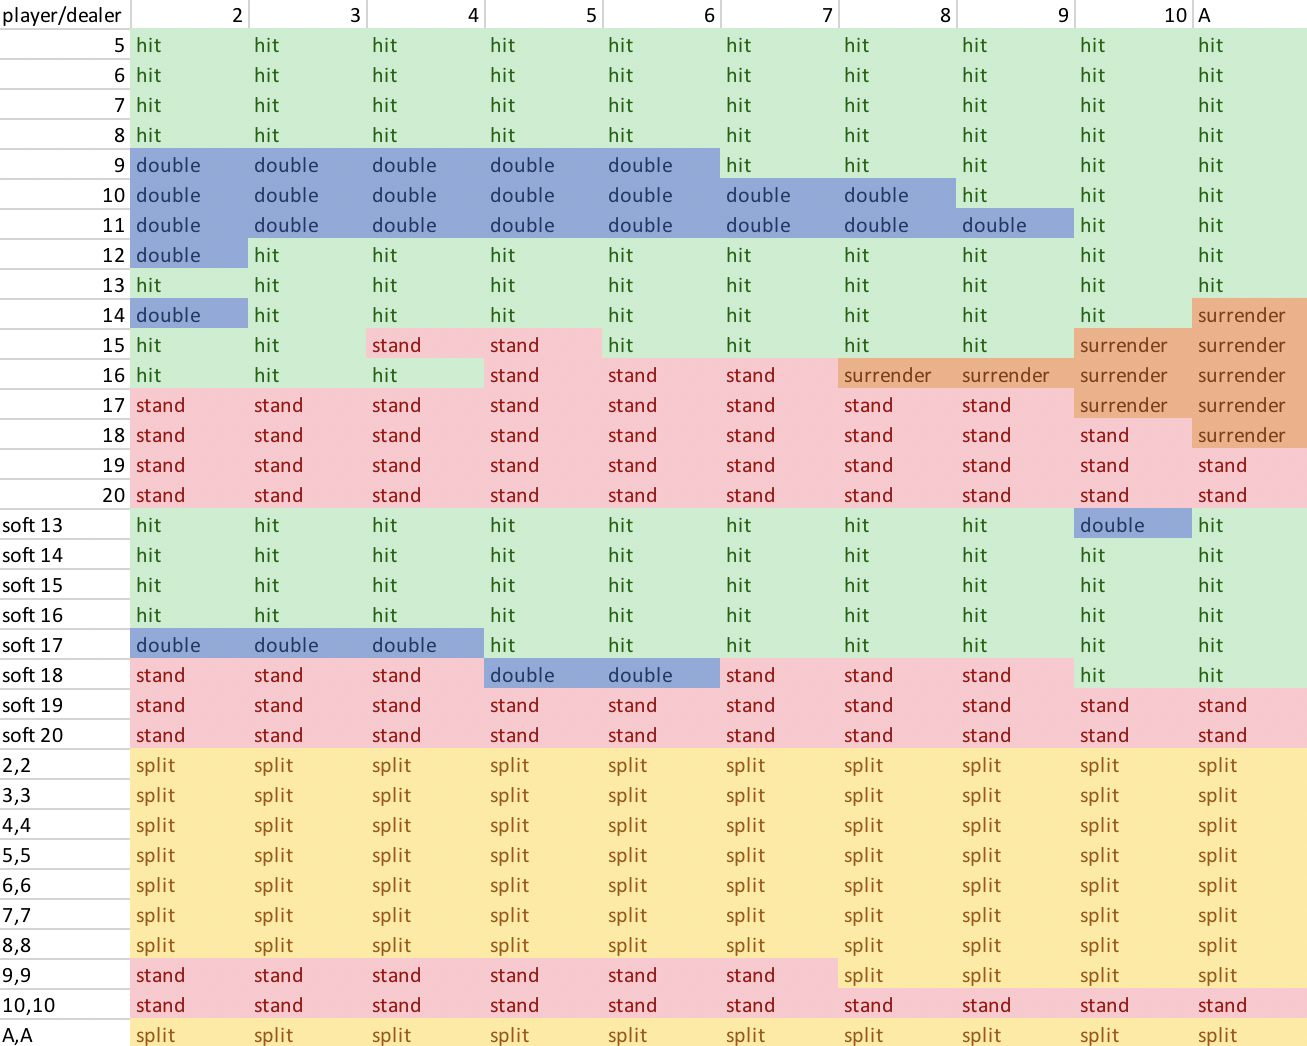
\includegraphics[width=\textwidth]{model_chart}
		\caption{Derived policy}
	\end{subfigure}
\end{figure}
\FloatBarrier

We can see that our agent learns the structure of the game pretty well, but doesn't figure out exactly when it should double, split, and stand. Notably, our agent doesn't stand and double aggressively enough against the dealer's weak hands, and splits too frequently against the dealer's strong hands\footnote{Intuitively, hands close to 10 are strong because the most common draws are 10s and 11s, and hands around 15 are weak because they break quite often.}. This suggests that our exploration method and hyperparameters could use some more tuning. 

\section{Conclusion}

Ultimately, although we were able to learn a good policy for blackjack, we were unable to learn the optimal policy. This result is surprising, as blackjack is small game compared to domains like go and Atari that deep reinforcement learning has already mastered. However, it seems the deep $Q$-learning has some trouble learning probabilistic transitions and rewards, at least those centered around thresholds like the ones in blackjack. Further, it seems that deep $Q$-learning's neural network approximation loses some precision. 

Nonetheless, it should be noted that our model is relatively primitive. It seems likely that after adapting recent innovations to deep $Q$-learning and with some more sophisticated tuning and hyperparameter search, we could likely find the optimal policy. We could also consider alternative state space formulations or network structures that might fit better together. Still, even in this setting, deep $Q$-learning significantly outperformed traditional $Q$-learning despite training for an order of magnitude fewer episodes and storing far fewer parameters. It's clear that deep $Q$-networks and similar neural models represent the future of reinforcement learning. 

\section{Code}

Our code and the source for this paper can be found at this GitHub repository: \url{https://github.com/nalkpas/CS230-2018-Project}

\subsubsection*{Acknowledgments}

Thanks to Zach Barnes for his mentorship, to the rest of teaching staff for a fun quarter, and to Volodymyr Mnih and everyone else at DeepMind for revolutionizing playing games. 

\section*{References}

\small

[1] Silver, D.\ \& Hubert, T.\ \& Schrittweiser, J. (2017, December 5). \textit{Mastering Chess and Shogi by Self-Play with a General Reinforcement Learning Algorithm}.

[2] Silver, D.\ \& Huang, A. (2016, January 28). \textit{Mastering the Game of Go with Deep Neural Networks and Tree Search}.

[3] Mnih, V.\ et al. (2013, December 19). \textit{Playing Atari with Deep Reinforcement Learning}.

[4] \url{https://en.wikipedia.org/wiki/Blackjack#History}, last accessed March 22\textsuperscript{nd}, 2018

[5] Baldwin, R.\ et al. (1956, September). \textit{The Optimum Strategy in Blackjack}.

[6] Melrose, R.\ \& MacGlashan, J.\ \& Tellex, S. (2017, November 20). \textit{Implementing the Deep Q-Network}.

[7] Paszke, A. (2017, May 2). \textit{Reinforcement Learning (DQN) tutorial}. \url{http://pytorch.org/tutorials/intermediate/reinforcement_q_learning.html}, last accessed March 22\textsuperscript{nd}, 108. 

\end{document}
